\chapter*{Введение}		
\addcontentsline{toc}{chapter}{Введение}	%добавляем в оглавление			
FAINA - численный код, предназначенный для расчетов различных видов электромагнитного излучения от астрофизических источников. Код написан на языке C++ с использованием только стандартной библиотеки. В текущей версии кода реализованы следующие виды излучения: синхротронное излучение, излучение за счет обратного комптоновского рассеяния, излучение распада пионов в результате свободно-свободных столкновений протонов, а так же тормозное излучение. FAINA позволяет вычислять наблюдаемые потоки от источников с заданными параметрами, а так же вычислять параметры источников с помощью фитирования наблюдаемых данных расчетными. Так же возможен учет эволюции источников и их излучения во времени.

\section*{Установка и запуск}
\addcontentsline{toc}{section}{Установка и запуск}
Текущая версия кода доступна на github https://github.com/VadimRomansky/Faina. Скачайте архив и разархивируйте его в директорию Faina.
\subsection*{Windows}
\addcontentsline{toc}{subsection}{Windows}
Для работы с кодом и его запуска в операционной системе Windows необходимо использовать Microsoft Visual Studio и открыть с помощью неё файл Faina.sin, содержащийся в корневой директории кода. Работоспособность проверялась на версии Visual Studio 2022.
\subsection*{Linux}
\addcontentsline{toc}{subsection}{Linux}
Для запуска FAINA в операционной системе Linux предусмотрены два варианта. Рекомендуется использовать среду разработки QtCreator и открыть с помощью неё проектный файл Faina.pro, содержащийся в корневой дирректории кода. 

Так же возможна непосредственная компиляция и запуск из терминала, с помощью комманд
\begin{lstlisting}[language=bash]
	$ g++ -o faina *.cpp
	$ ./faina
\end{lstlisting}
\section*{Быстрый старт}
\addcontentsline{toc}{section}{Быстрый старт}
Рассмотрим простейший пример, приведенный в процедуре evaluateSimpleSynchrotron в файле main.cpp. В данном примере рассмытривается синхротронное излучение от однородного источника в форме плоского диска, с заданной степенной функцией распределения излучающих электронов. Сначала зададим значения магнитного поля и концентрации электронов (в коде используются единицы СГС).

\begin{lstlisting}[language=c++]
	double B = 1.0;
	double electronConcentration = 1.0;
\end{lstlisting}

После этого нужно создать распределение электронов. Вычисление синхротрона реализовано только для изотропного распределения, поэтому создадим изотропное степенное распределение. Конструктор степенного распределения принимает следующие параметры: массу частиц, подставим константу - массу электрона, степенной индекс (он считается положительным и должен быть больше 1), энергию, с которой начинается спектр, в качестве нее выберем энергию покоя электронов, и концентрацию электронов.

\begin{lstlisting}[language=c++]
	MassiveParticleIsotropicDistribution* distribution =
	new MassiveParticlePowerLawDistribution(
	massElectron, 3.0, me_c2, electronConcentration);
\end{lstlisting}

Далее создадим источник излучения - однородный плоский диск, парметры его конструктора это распределение электронов, магнитное поле, синус угла наклона магнитного поля к лучу зрения, радиус, толщина и расстояние до него.

\begin{lstlisting}[language=c++]
	RadiationSource* source = new SimpleFlatSource(
	distribution, B, 1.0, parsec, parsec, 1000 * parsec);
\end{lstlisting}

Последнее, что нам нужно - вычислитель потока излучения. Ему нужно указать рассматриваемый диапазон энергий электронов, в виде числа точек разбиения для интегрирования, минимальной и максимальной энергии. Так же есть параметр, отвечающий за учет синхротронного самопоглощения, по умолчанию его значение true.

\begin{lstlisting}[language=c++]
	RadiationEvaluator* evaluator = new 
	SynchrotronEvaluator(1000, me_c2, 1000 * me_c2, true);
\end{lstlisting}

Синхротронное приближение применимо только при частотах, намного больших циклотронной, поэтому вычислим её

\begin{lstlisting}[language=c++]
	double cyclOmega = 
	electron_charge * B / (massElectron * speed_of_light);
\end{lstlisting}

Теперь осталось только вычислить само излучение. У класса RadiationEvaluator есть метод, вычисляющий поток излучения в заданном диапазоне энергий и записывающий его в файл. Нужно указать имя файла, источник излучения, минимальную и максимальную энергии фотонов, и желаемое количество точек в этом диапазоне. Вычисление потока и вывод происходит в единицах энергия фотонов - энергетическая плотность потока излучения $\text{Вт}/ \text{эрг } {\text{см}}^2 = {\text{см}}^{-2} {\text{c}}^{-1}$. Если необходим вывод в других единицах, то запись в файл нужно переписать самостоятельно. 

\begin{lstlisting}[language=c++]
	evaluator->writeFluxFromSourceToFile("out.dat",source, 
	10*hplank*cyclOmega, 1E5*hplank*cyclOmega, 1000);
\end{lstlisting}


Функция вычисления синхротронного потока источника готова, осталось лишь вызвать её из основной процедуры main(). В результате вычисления должен получиться спектр источника, показанный на рисунке \ref{example0}
\begin{figure}
	\centering
	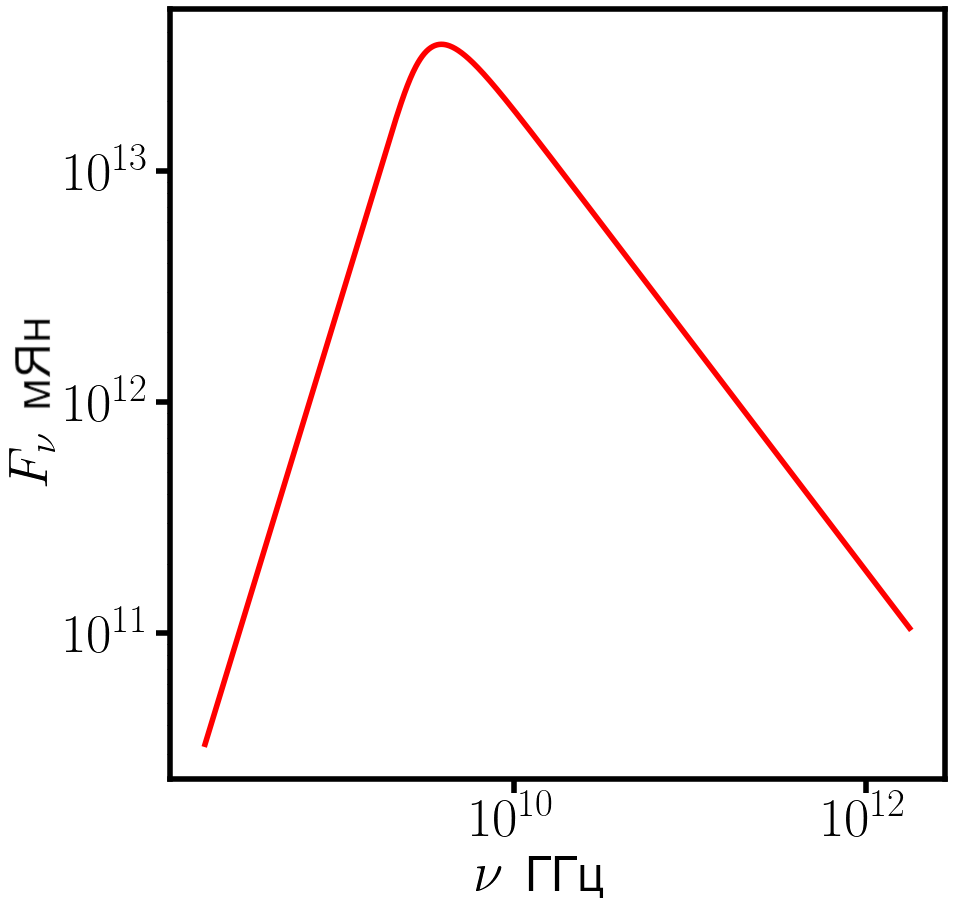
\includegraphics[width=12.5 cm]{./fig/example0.png} 
	\caption{Энергетическая плотность потока синхротронного излучения от тестового источника}
	\label{example0}
\end{figure}